\section{Discussion}
\label{sec:discussion}

\begin{itemize}
\itemsep0em
\item results that are contradictory
\item results that data suggests that is wrong
\item a better way to measure and offer broadband based on utilization?
\end{itemize}


\subsection{User Taxonomy}
\label{subsec:taxonomy}


\begin{figure}[ht!]
\begin{minipage}{0.9\linewidth}
\centering
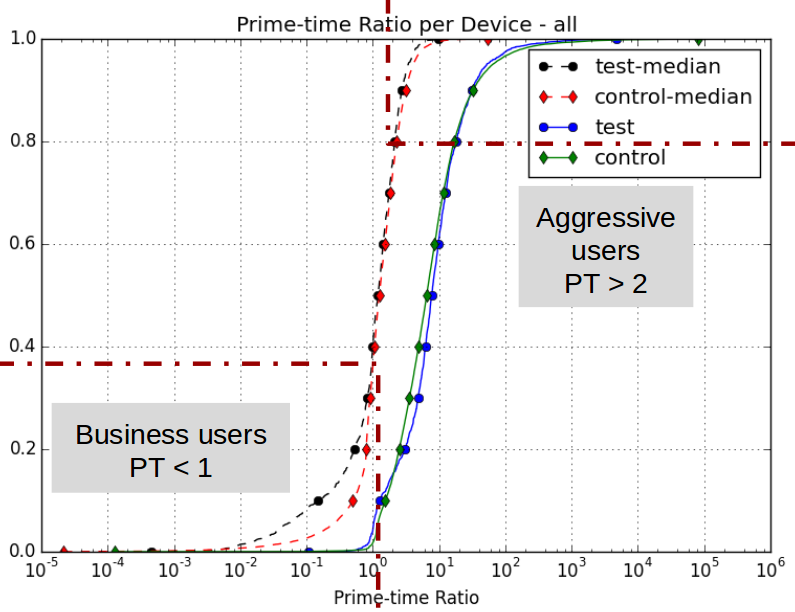
\includegraphics[width=0.9\linewidth]{figures/cdf-prime-time-ratio[replace].png}
\caption{(old) Prime Time ratio + usage can be used to divide users into four sets: aggressive all time + non aggressive all time, aggressive peak time, aggressive non-peak time (business hours))}
%http://riverside.noise.gatech.edu:8083/separated/full/cdf-prime-time-ratio-per-device.png\\
%http://riverside.noise.gatech.edu:8083/plots/full_dw/prime-time-ratio-per-device-cdf-ALL.png
\label{fig:CDF-prime-time-ratio}
\end{minipage}
\end{figure}

\begin{itemize}
\itemsep0em
\item Figure ~\ref{fig:CDF-prime-time-ratio}
\item Sandvine does it by real-time entertainment usage
\begin{itemize}
\item  cord cutters (> 85\%ile): uses 11 times more data than the rest
\item typical subscriber
\item non streamers (< 15\%ile): uses just 0.5% of total data per month
\end{itemize}
\item the segregation splits business and casual users based on usage and motivates our discussion on multiple benchmarks based on usage.
\item 30\% PT $<$ 1: possibly businesses with normal work-hours
\item 20\% PT $>$ 2: aggressive prime-time streamers
\item taxonomy: aggressive all time + non aggressive all time, aggressive peak time, aggressive non-peak time (business hours)

\end{itemize}




\todo{ TO PLOT :}
\begin{itemize}
\itemsep0em
\item peak ratio cdf vs no of devices
\item peak ratio cdf vs time of day where peak occurred
\item no of devices cdf vs time of day where peak occurred
\end{itemize}
